\documentclass{article}
\usepackage[T1]{fontenc}
\usepackage{lmodern}
\usepackage{graphicx}
\usepackage{amsmath,amssymb}
\usepackage[a4paper,margin=2cm]{geometry}
\usepackage[absolute,overlay]{textpos}
\setlength{\TPHorizModule}{1mm}
\setlength{\TPVertModule}{1mm}
\usepackage[indonesian]{babel}
\usepackage{hyperref}
\setlength{\emergencystretch}{2em}
% unit: Halaman 7

\begin{document}

% === Halaman 7 (python/native) ===

• Nilai entropi berkisar dalam rentang:

• Entropi minimum = 0 bit

   → Tidak ada ketidakpastian

   → Terjadi jika hanya ada satu simbol dengan peluang 1 (pasti).

   Contoh: n = 1, misalkan A dan p(A) =1  → H(X) = −1⋅log2 1=0 

• Entropi maksimum = log2(n) bit

   → Terjadi jika semua simbol muncul dengan peluang sama, yaitu 1/n.

   → Ketidakpastian paling tinggi, setiap simbol membawa informasi maksimal. 

   Contoh: Empat simbol dengan peluang sama (0.25) →

7

% deskripsi: gambar native xref 51
\noindent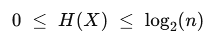
\includegraphics[width=0.85\textwidth]{../../images/python/page_007_img_01.png}

% deskripsi: gambar native xref 52
\noindent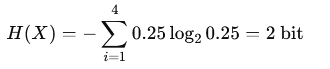
\includegraphics[width=0.85\textwidth]{../../images/python/page_007_img_02.png}

\end{document}
